\section{Halo-indepdent measures of baryonic flows}
\label{sec:haloindependent}

\begin{figure*} \centering
	\includegraphics[width=\textwidth]{figures/kspafig.pdf} \caption{A
	diagrammatic representation of the distance measure. On the left, the
	initial conditions are shown. The blue dark matter particles each find
	their closest dark matter and gas (red) neighbour. These particles are
    then tracked to the final state of the simulation at z=0 (right) and the
    distance between them calculated again to assess the relative motion of dark
    matter and baryons.} \label{fig:distancemeasure}
\end{figure*}

\subsection{Using inter-particle distances to describe transfer}

Usually, analysing how baryonic and dark matter move differently requires the
use of a halo finder, to identify structures between which gas can flow.
However, if the gas and dark matter become decoupled, it should be possible to
see this effect without having to consider bound structures at all.

To find how separated the dark matter becomes from the gas, two distances
\emph{in the final snapshot at $z=0$} are considered. First, the distance
from each dark matter particle to the corresponding closest dark matter
neighbour in the \emph{initial conditions}, i.e. the distance
\begin{equation}
    r_{ij, ~z=0} = \sqrt{ \left| \mathbf{x}_{i,
    ~z=0} - \mathbf{x}_{j \ni \min(r_{ij, ~z=z_{ini}}), ~z=0} \right|^2 }
    \label{eqn:minimal}
\end{equation}
where $\mathbf{x}_i$ is the position of particle $i$, and $\mathbf{x}_i -
\mathbf{x}_j$ is wrapped within the periodic box. The corresponding distance
between the dark matter particle and the closest gas neighbour in the initial
conditions is also considered, $r_{\rm gas}$. A diagrammatic representation of
this is given in Figure \ref{fig:distancemeasure}. Star particles at $z=0$ are
ID matched with their gas progenitors, where at all possible. 

\subsection{Distribution of Distances}

\begin{figure} \centering
	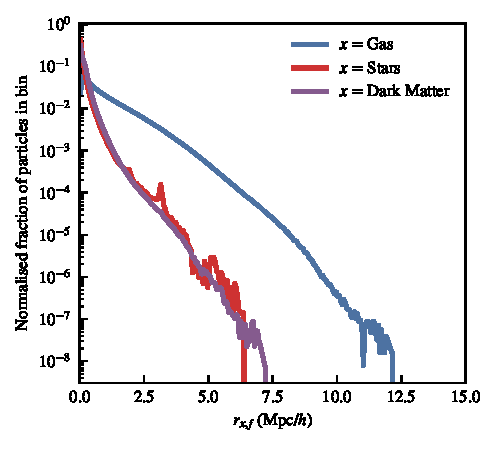
\includegraphics[width=\columnwidth]{generated_figures/neighbour_analysis_simple_histogram.pdf}
	\caption{The distribution of all distances to particles at $z=0$. Note
	the similarity between the dark matter distribution and the stellar
	distribution, and how different they are to the gas with the associated
	long tail.} \label{fig:alldistances}
\end{figure}

Now that the distances at $z=0$ have been identified it is possible to
compare how mixed the dark matter has become, compared to the gas, beginning
with the distribution of final particle distances from their initial
neighbour. In Figure \ref{fig:alldistances} the similar dynamical
distributions of the stellar and dark matter components are shown, with the
gaseous component having a significantly longer tail. By the end of the
simulation, gas particles can end up around $15\hmpc{}$ away from their original
nearest neighbour; this can only occur due to the strong wind velocities that
are powered by the AGN in the simulation.

Such a large separation is certainly possible over the course of the
simulation in the \simba{} model. AGN winds are powered at around $10^4
\kms{}$, meaning that over the whole run-time of the simulation the maximal
distance that a wind can travel is nearly 150 Mpc; enough to wrap the whole
box three times. This is, however, clearly an extreme upper limit, with the
AGN winds being slowed immediately by interaction with the potential well of
the halo.

The similarity between the dark matter and stellar distribution is clear
here. Both follow extremely similar power-laws, something that must be
investigated further in the future. That the stars must form out of particles
that were initially gas in the simulation is nontrivial. The similar
distribution could simply owe to the dynamics of the gas that eventually
forms stars being dominated by gravitational forces, or the mixing timescale
being short enough that the majority of the stars become well mixed with the
dark matter by the end of the simulation. This could also possibly be a
signature of the gravitational softening, or be a signature of tidal
stripping of satellite halos, now thought to be a significant effect, as was
shown by \citet{vandenbosch2018}.

\subsection{Particle-by-particle comparison to dark matter}

\begin{figure} \centering
	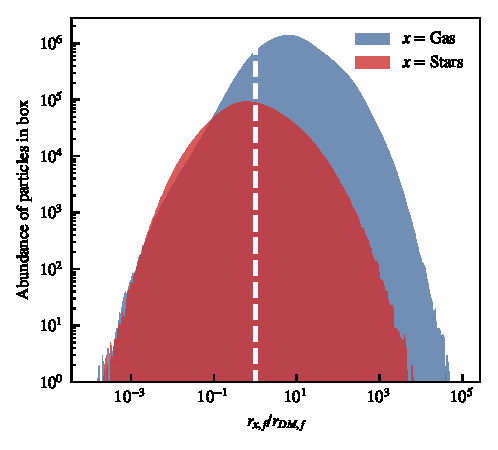
\includegraphics[width=\columnwidth]{generated_figures/neighbour_analysis_ratio_histogram.pdf}
	\caption{The distribution of relative final state distances for each
	dark matter particle to the appropriate gas and stellar (these
	correspond to $i$ in the bottom label) particles at $z=0$ normalised by
	the distance to the dark matter particle that was closest in the
	initial conditions. Note the significantly different distributions for
	gas and stars.}
\label{fig:dmvsstarvsgas} \end{figure}

Comparing solely the distributions of each particle type prevents the use of
the fine-grained particle data that is available. It is possible to compare,
for a given dark matter particle in the initial conditions, how much the
nearest baryonic particle has moved, compared to the nearest dark matter
particle. For each particle, the distance that the nearest dark matter
neighbour has travelled, compared to the nearest baryonic neighbour, is plotted in
Figure \ref{fig:dmvsstarvsgas}. The stellar distribution is highly symmetric
and peaks around $r_{\rm star}/r_{\rm DM} = 1$, implying that the stellar and
dark matter components have a very similar dynamical distribution (see also
Figure \ref{fig:alldistances}) but that this is not a \emph{local} effect.
The gas and dark matter do not become separated from the gas, as implied by the
original histogram, causing this effect; the stellar and dark matter are both
mixed in a similar way by the gravitational dynamics, completely randomly. If
there was a local effect here, we would see that the ratio of
$r_{\rm star}/r_{\rm DM}$ would be much more tightly constrained.

The same distribution for the gas, however, has a different signature.
$r_{\rm gas}/r_{\rm DM}$ peaks around 10, not 1, showing that gas ends up
preferentially further away than the neighbouring dark matter particle. That
gas behaves differently to dark matter is unsurprising; gas particles feel
repulsive forces from hydrodynamics, can be heated, and even get blown out of
galaxies. The strength of this effect, to blow gas out to distances of around
$\sim15 \hmpc{}$, corresponds approximately to the size of superbubbles in the
IGM created by AGN, suggesting that this is a signature of feedback
\citep{dave2018}. The effect of the gravitational dynamics can not be
decoupled from this result; the 9 orders of magnitude wide distribution is
also affected by mixing in the dark matter. The specific details of the
dynamics that causes this spread is still not understood, and must be
investigated in further work.
